The main design points to focus on going forward are:
\begin{itemize}
\item OpenGL Rendered Output and Fully Interactive Interface
\item Separate Threads for Simulation and Graphics/Interface
\item The user Set-up of Scenario
\item The user is able to save and load scenarios to and from the file-system.
\item The user is able to modify variables in the simulation
  \begin{itemize}
  \item Mass of Bodies
  \item Position of Bodies
  \item Velocity of Bodies
  \item Radius of Bodies
  \item Gravitational Constant
  \item Simulation Time Step
  \item Iterations Per Frame
  \end{itemize}
\item It will be necessary to synchronise the threads in a way that limits the speed that the simulation can run at to the update speed of the renderer, which will likely be the bottleneck at low body counts.
\item Target frame-rate for the display should be 60FPS to maintain a smooth interactive experience.
\end{itemize}

\subsection{Threading}
\paragraph{}
The threaded nature of this program lends itself extremely well to modular design, as new threads are assigned a thread from which they start, effectively becoming their own 'main' function.

\paragraph{}
The main difficulty when working with multiple threads is ensuring that they are well synchronised as to prevent race conditions, these occur when one thread completes a task before another which could lead to incorrect program execution. A similar issue is when working with shared data, multiple threads writing to the same data will cause exceptions in the program; reading data while it is being written may not throw an exception, but it will cause errors.

\paragraph{}
The main way that this will be dealt with this is to implement locks, these are variables that are written before a thread accesses certain data, another thread attempting to write to the data must first check the lock variable to ensure that data is free to write. Once a thread is done, the lock variable is cleared and another thread is safe to write to the shared data.

\paragraph{}
The benefits of using threading means that while one part of the program is managing a time consuming task such as rendering the display, the simulation can still be running on another thread, thus significantly improving the performance of the program by ensuring that the program is making the best possible use of time.

\paragraph{}
When it comes to the actual scenario containing body information, each thread will have its own local copy of the scenario, at the beginning of a simulation or graphics loop copy their current data to respective shared access stores, threads also have their own status 'registers' in shared memory area and can change bits in these variables to denote their current status throughout their execution path. In the case of the graphics and interface thread, the thread will turn on a certain bit in its register when it has received user input and a change has been made, when the simulation thread gets to this point it will read this bit and copy the changes to its local storage. This algorithm is best explained using a state transition diagram due to its branched complexity. Another method of locking the variables that may end up somewhat cleaner is to make use of Mutual Exclusion Objects; these are a feature of C++ which would produce a similar result to the prior explanation, they are however implemented in the compiler itself.

\paragraph{}
In short, thread safety will be ensured through the use of Thread-Local Storage (TLS) and locks on any shared data to prevent concurrent writes/reads. Thread registers will also be found in shared data describing the current state of a thread and its current task, as well as flags denoting new available data or requests for new data. The system will make use of a basic request > acknowledge system to ensure that it is correctly synchronised at all times. When the status registers are included. This means that the thread also has the ability to be re-entrant, allowing it to resume should the thread be interrupted.

\paragraph{}
In order for this re-entrancy to work correctly, the graphics processing and handling must be done on the initial thread, as the OpenGL wrapper library (GLFW) states that the OpenGL code is not thread-safe. (i.e. not re-entrant) The simulation component can then be handled in a secondary thread and can provide new simulation data to render into the shared data area, as well as setting register bits to denote that new data is available, when the render thread sees that new data is available, it will set its own bits to acknowledge that it has taken the new data, on the next loop, the simulation thread will clear its new data bit if the render thread has acknowledged and will eventually repeat the process, If for some reason the rendering is taking longer than usual and the new data has not been taken by the next loop the simulation thread will sleep until the new data has been taken, meaning that there is a small 1 deep buffer for the scenario.

\paragraph{}
It may be beneficial to implement a larger buffer for the simulation so that it can build up a backlog of new data frames to improve performance, however this is not a priority as if user input is given the backlog would need to be discarded, meaning that this would only provide a performance gain should no changes be made by the user, and only if the simulation is running much faster than the renderer.

\paragraph{}
Another point for consideration is the actual parallelisation of the simulation, while currently the simulation is broken up into its own thread the carries out computations for all bodies, it would be possible to split the simulation itself onto multiple threads to improve the simulation speed further by running computations for each body on an individual thread, this would result in some duplication of calculations but the sign does not need to be reversed later on.

\paragraph{}
On a similar note, this same idea of parallelisation can be expanded much further, while an average consumer CPU may have the ability to run 4 concurrent threads, with high end servers supporting multiple processors with capability of upwards of 36 threads each. This still somewhat pales in comparison to GPUs which can have hundreds or even thousands of compute cores. These are built for crunching numbers; the cores are far simpler but can carry out similar tasks to the main processor. The difficulty comes in accessing them because there are several different manufacturers of graphics processors with vastly different software interfaces. 

\paragraph{}
OpenCL is an API that allows easier access to the graphics processor and leverage the computing power that is available in them. When code is written in a particular and correct way and the memory of the graphics card is managed correctly, performance gains can be huge. The disadvantage to this system is that it tends to require dedicated graphics hardware as opposed to integrated graphics, as integrated graphics processors will have a far lower amount of cores; it would also likely dramatically affect the performance of the rendering of the scene.

\paragraph{}
The main issue that presents itself with GPU calculation is that in order to get the large improvements to performance you are limited to using single precision floating point arithmetic, this reduces the maximum attainable precision of the simulation as well as limiting the effective size that is possible. There are specialist GPUs that exist which are built with double precision floating point, these are extremely expensive and out of the reach of most people and establishments.

\paragraph{}
Because of the low amount of bodies that are likely to be used in this simulation, I do not plan to implement either CPU Simulation parallelisation or OpenCL based parallelisation as it is unlikely to be something that most people will be able to leverage and gain an effective performance benefit without a dedicated high end PCI-E graphics card. Along with implementing the Barnes-Hut simplification algorithm it could make for an interesting extension task.

\subsection{Libraries}
\paragraph{}
Libraries will be a critical part of the programming and code structure for this project, both third party and self-programmed.

\paragraph{}
The first and most obvious library is GLFW, a minimal wrapper that allows for the creation of OpenGL contexts which can be used to render graphics. It also provides easy access to inputs from keyboard and mouse. The benefit of this library is that is provides an extremely lightweight abstraction layer for doing all of these things across different OS platforms, making it far easier to port code from one platform to another.

\paragraph{}
The main reason for this is that setting up windows for displaying OpenGL contexts can be somewhat involved when it comes to writing operating system specific code, not something that is particularly necessary in this application. The library also provides full access to keyboard and mouse inputs which are critical to the operation of the program and are another feature that would normally require a large amount of somewhat messy operating system specific code, making porting to different target systems somewhat difficult.

\paragraph{}
Another library that will be used is AntTweakBar, this library provides a quick and simple to use utility for exposing certain variables and information to the user through a variety of control methods such as buttons and sliders for setting variables to particular values. It also provides a good way of displaying textual information to the user such as a basic help screen.

\paragraph{}
The C and C++ standard libraries will also be used in this program; these contain functions that allow the use of input and output streams as well as some higher level features such as string handling, threading and vectors, the main two here are threading and vectors. The threading library provides an object orientated implementation for threads, while vector provides an object orientated implementation of a dynamic collection, or array that can change size during program runtime.

\paragraph{}
The library structure can also be used for my own code in order to split it up, code can be split into separate code files (.c / .cpp) and linked together using header files (.h / .hpp), these files contain function prototypes for functions that reside inside the code file that it describes. The benefit of this is that the function prototypes are not required inside the code file. It also means that header 'guards' can be used in order to prevent the code being duplicated at the link stage.  The result of this is much cleaner code that is much easier to reuse in other projects.

\paragraph{}
When it comes to the compilation and linking of programs, there are generally two methods to this for libraries, static and dynamic, while static linking will link all of the library code into the application file, dynamic relies on libraries being compiled ahead of time and being shipped with the application or as redistributables, which the user can install to their system and any application that makes use of them can in theory make use of the existing library rather than needing its own copy.

\paragraph{}
The benefit of dynamic linking is that the final size of the application file is much smaller, it also means that libraries do not need to be compiled alongside the application, reducing the time to compile a fresh copy of the target application. The disadvantage is that more files are required to be placed alongside the application or added to a system directory which requires installation. It can also result in lower resource usage if multiple applications use the same libraries.

\paragraph{}
In the case of this project, static linking is a more attractive option, as while the size of the executable is somewhat larger, other files are not required and the executable can be placed anywhere and run without the need for other external files. When looking at compile time, parts of code that are compiled generally only need to be recompiled if those parts of code change as object files are retained, meaning that compile time reductions are likely to be minimal when going with the dynamic approach.

\subsection{Structure}
\paragraph{}
This program has two main identifiable components, the simulation and graphics/interface, because these parts are sufficiently different from each other, it makes sense to split the processing into threads, potentially making code more readable but also providing the potential for some performance improvements.

\subsubsection{Overall System Design}
\import{tables/}{3_overallsystem.tex}

\paragraph{}
The basic layout of the program is an Input -> Simulate -> Render loop, however in order to produce an output that is actually useful a certain amount of management must be in place to control how much simulation time passes in each frame, meaning that the simulation will only calculate a number of iterations per frame.

\paragraph{}
GLFW and OpenGL are not handled using object orientation, and instead are handled in a more traditional procedural way. Input in GLFW is handled through the use of callback functions, these must be setup by calling a particular library function and passing it a programmer-defined function that can accept specific attributes that relate to that particular input. (Listed in GLFW Documentation) At the time that that particular input is received that function will be called and the variables passed to it reflect the input given. (Happens at call of GLFWPollEvents(); in render loop.)\\\

\begin{center}
\ttfamily{glfwSetCursorPosCallback(\color{red}window\color{black}, cursorPosCallback);}\\\
\end{center}

When GLFWPollEvents(); is called, the function cursorPosCallback(); will be called if the mouse moves in the GLFW window and its window coordinates will be passed to the function which can then handle any programmer-defined actions with that data.

\paragraph{}
The interface will be constructed using input taken from GLFW, these input events will contain a check which passes the control onto the check function for the main interface library, AntTweakBar. This ensures that the inputs are available to both components, even though there is a degree of separation between them.
Unfortunately it is not possible to have assign callback functions to class-member functions, this is something that would make organisation somewhat easier.

\paragraph{}
While the rendering and interface will be mostly programmed using callbacks and procedural programming, however the simulation; due to its nature of distinct bodies or objects, is extremely well suited to an object orientated method of programming.


\pagebreak
\subsubsection{Program Flowchart}
\begin{figure}[!ht]
  \centering
  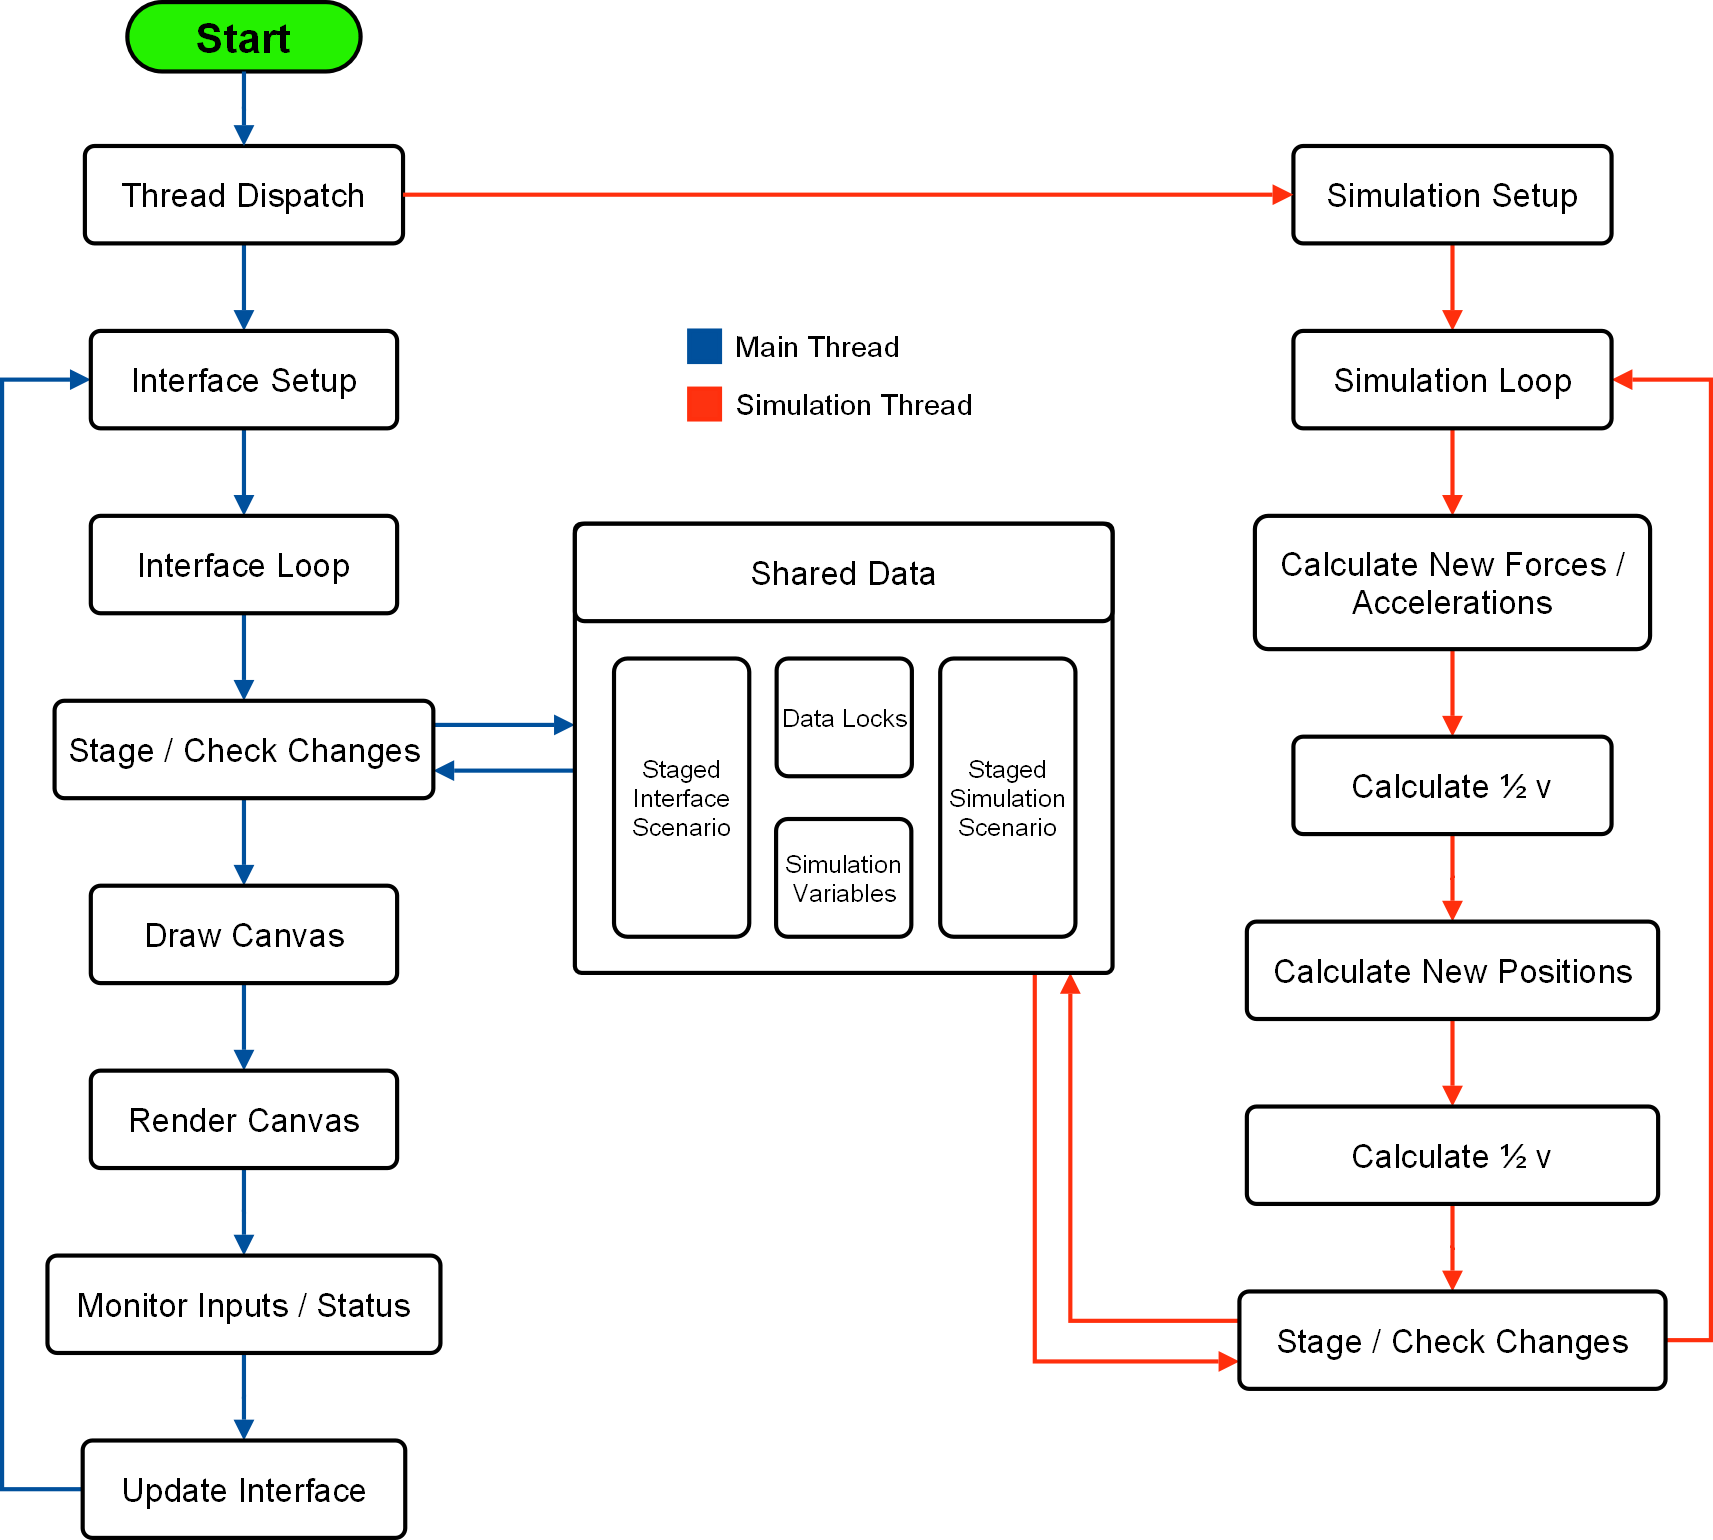
\includegraphics[width=\textwidth]{img/flowchart.png}
  \caption{System Flowchart}
\end{figure}

\pagebreak
\subsubsection{Algorithms}
\import{sections/design/}{algorithms.tex}

\pagebreak
\subsubsection{Data Range and Validation}
The main issue with the validation of data is that it does not play particularly nicely with the medium of the simulation, which is Space, in reality, an orbit is massive because the size of the bodies and their velocities are massive, for example, the earth orbits about 149.6 million kilometres from the sun and at a velocity of 29.78 kilometres per second. The (current) furthest known common body in our solar system, Pluto, orbits at a range of 4.4-7.4 billion kilometres and at a velocity of only 4.67 kilometres per second.

\paragraph{}
The main issue here is the range of distances; from this view it makes it quite difficult to set limitations of the simulation because of the simple fact that space is vast and distances are vast. It is however necessary to take into account that this scale would also not be practical in the simulation as it would be nearly impossible to make out individual bodies inside an accurate solar system model. (The earth has a radius of just 6,371 kilometres.)

\paragraph{}
There is also the issue that when bodies are two close together and the velocities are too great, the simulation method will breakdown; even with the improved Leapfrog method for integrating the acceleration, meaning that the scale of the simulation cannot be confined to being too small.

\paragraph{}
In terms of massive scale, something to look out for is the loss of precision when the numbers get too big, because the simulation will make use of the double floating point data type, as with float precision is not constant through a range in numbers as the mantissa is taken up by the most significant bits in a large number. C++ implements a IEEE variant of double-precision floating point, a 64 bit variable, 1 sign bit, an 11 bit exponent and a 52 bit fraction. (IEEE 754) (There are some other differences compared to twos complement floating point.)

\paragraph{}
These bit depths mean that (depending on particular implementation) the double precision type has 15-17 digits of precision, this would be enough digits to describe the position of Pluto in our solar system, and still have about 5 digits of precision remaining for the decimal, one problem with this is that the force that is provided by other bodies in the solar system could be quite small and result in a cancellation error in calculation that does not take into account the smaller forces, this will increase the error in the simulation. However due to the size and mass of bodies in our solar system all of the interactions are still likely to be within range of each other and only a few powers of ten apart, meaning that it is still something that is possible to calculate without cancellation the most significant bits.

\paragraph{}
There will however be cancellation when it comes to the calculation and use of the mass of bodies, for example, the sun has a mass of $\num{1.989e30} kg$, this is easily possible to represent however there will be very little precision, only the first 15 most significant powers of ten change will have any effect to the mass (i.e: anything with a mass of less than $\num{1e15} kg$.). In the grand scheme of things this is not a problem that is likely to have much of an effect on the simulation, especially at the scale that will be likely to be used.

\paragraph{}
The force that the sun exerts on Pluto at its highest point results in a change in acceleration of $\num{2.42e-6}$, at this height Pluto is orbiting at $3.71 kms^{-1}$, while this will be in range and not result in cancellation, when looking at the force exerted by the relationship between Earth and Pluto, the change in acceleration is $\num{7.05e-12}$, this is only just within the range of the double precision when added to the velocity of Pluto, which is orbiting quite slowly to begin with.

\paragraph{}
Due to the nature of a n-body system, it is impossible to predict the outcome over a period of time, while a two body system can be described perfectly (in an ideal sense) with equations, an n-body system cannot, and will generally become chaotic over a relatively short length of time. This again makes it something that is difficult to place validations and limitations on, as a lot of possible restrictions could end up crippling the usage of the program in certain scenarios.

\paragraph{}
It may make a certain degree of sense to look at the maximum distance that can be represented using a double variable yet still maintain a certain number of decimal places for the precision of the calculations (At least 2). This would mean that assuming a base unit of 1 meter, and a precision of 15 digits, the orbit of Pluto can still be represented on a centimetre scale and still have orbits further out.

\paragraph{}
Worth noting is that there will be a fair amount of error due to the way that decimals are represented in binary. For example, it is generally not possible to exactly represent …0.01, and it will instead be represented as …0.00996, the rest of the digits are due to the implementation that is used both by the compiler and the hardware being used. This will result in an error that can accumulate, adding to the potential for chaos and other miscalculation errors in the simulation. 

\paragraph{}
While this would work as detached simulation engine without a rendering counterpart, the inclusion and requirement of a graphical front-end and display for the results of the simulation places another limitation on the available range. This is because rendering at a hardware level, handled by a GPU is carried out using single precision floating point, with only high-end GPUs having any kind of FP64 capability and these are generally suited to raw compute rather than actual graphical rendering.

\paragraph{}
When taking this into account, standard float has only 7 digits of precision, meaning that when representing the orbit of Pluto, you only end up with a precision in the range of 1000 km which is a considerable distance on a smaller scale, it also makes things like rendering an accurate circle of smaller radius somewhat difficult, especially when you consider that the radius of Pluto is only 1186 km. (The circle drawing algorithm discussed later on will end up drawing a square.)

\paragraph{}
In order to improve the minimum precision that the renderer will encounter in order to preserve accuracy, the maximum distance that a body can be from the origin must be reduced, reducing by an order of magnitude will reduce the absolute maximum to $\num{9.99E11}$ m, which is only enough to represent out to past the orbit of Jupiter, while this is quite a drop in the maximum distance, it will make the precision of the simulation much higher at its maximum extremes and also reduces the minimum render distance down to 100km, this makes a body the size of Pluto possible to render at the extremes. Because of the nature of floating point, smaller bodies can still be rendered, however they will not be visible after a certain distance due to the loss in precision. (They will however still be simulated; it could be a good idea to delete bodies that are smaller than a certain size after they travel too far or specify a minimum render size at the extents so that the body can still be selected by the user.)

\paragraph{}
Other more definite limitations include mass, which cannot be 0 or negative, while hypothetically possible, this would result in complications and odd behaviour in the simulation, something that is best to avoid. It makes little sense to implement any maximum for mass, as on a stellar scale, masses are extremely variable due to composition, type and size of bodies. (A good example of this are black holes, these are relatively small in size but super-massive.)

\paragraph{}
Maximum radius should also be limited, however it does once again bring up the issue of what makes sense, the sun in our solar system has a radius 696,000 km, while the largest known star, VY Canis Majoris reaches a staggering 1 billion km in radius (About 1420 Sol Radii), this actually be near the limit of the size of the simulation, making a body of this size quite pointless, a much more reasonable maximum would be 1 million km , allowing for representation of bodies somewhat larger than our own sun.

\paragraph{}
Other variables, such as time step, should be limited to being positive (It is however worth noting that the leapfrog integration method allows for time reversal, this requires some modification however.) so that time can only move forward. The number of iterations per frame should be limited to a range of 1 to 10000, while the upper range will likely be only run at target frame rate on extremely high end systems or with low numbers of bodies, this value will be the main control the user has for increasing the speed of the simulation without sacrificing on accuracy.

\paragraph{}
Gravitational constant should be constrained to being a positive number as a negative number would reverse the effects of gravity, the upper limit of the gravitational constant will be 10, with a lower limit of $\num{1E12}$.
Other values involved primarily in calculation, such as velocity and acceleration will not have the limitation set to the speed of light in vacuum, or $\num{3E8} ms^{-1}$. This is a law of the universe and cannot be bypassed. In reality it cannot be reached, as at relativistic speeds the mass of the approaching body will increase, this simulation does not cover relativistic effects. (Because these are vector quantities, the same limit exists for the negative range.) If a body reaches or exceeds this velocity it will be deleted.

\paragraph{}
I am still somewhat hesitant to implement limitations that are too stringent as it may result in a crippled simulation engine, however unlikely that its intended use is to reach those limits.

\paragraph{}
While all of the data is primarily numerical, notation such as 'E' ($\times10^x$) is likely to be used to make very large or small numbers easier to type. The numerical validation is by default handled by the AntTweakBar GUI and the data boxes will not accept text as they are defined variable types. While custom validation functions could be added by setting the variable type to string and manually reading and converting it, there are other areas where validation could be manually implemented. (This would only add extra overhead and reduce features.)

\subsubsection{Data Security and Integrity}
None of the data handled by the application is considered sensitive from a user sense, however all of the data is considered critical to the correct and accurate operation of the calculation. The main place that integrity is important is when it comes to sharing data between the simulation and the renderer, as both threads have the potential to be reading and writing to the same data, race conditions come into play and are likely to cause issues, such as reading data that is only partially updated. This area will be managed using a state machine like algorithm to ensure that data is written to and read at the correct times.

\paragraph{}
When it comes to the saving of scenarios, these files will be by default outputted to a directory alongside the main executable. The user will be able to choose the name of the saved file, if the file already exists, the user should be prompted to if they want to overwrite the existing data. On an expected exit of the program, the simulation data should be saved to a default storage file that keeps a backup of the last data in the program, this will be opened on start-up without prompt.

\paragraph{}
It is important that thread shared data is managed effectively so that there are no concurrent reads or writes as this will cause the corruption of data and potential issues further down the line in the event that a variable changes while another thread is reading the data. This can be managed via the use of \textit{Mutex} lock objects, if one of these are locked and another thread attempts to lock the same mutex it will pause until the locking thread unlocks the mutex, thus preventing concurrent read/write access.

\subsubsection{Data Record Structure}
The user has the ability to save the current state of the simulation, this will be stored in a file (.sav, text format) inside a sub-folder next to the application executable. The user has the ability to choose the particular name of the file.\\\

The data file must be able to store the following:

\begin{itemize}
\item Gravitational Constant
\item Simulation Iteration Time-step
\item Simulation Iterations per Frame
\item Number of Bodies
\item Simulation State Data
\item Body Storage (For Each)
  \begin{itemize}
  \item Mass
  \item Radius
  \item Colour
  \item Position (X, Y)
  \item Velocity (X, Y)
  \item Fixed
  \end{itemize}
\end{itemize}

\paragraph{}
The save file will only contain data which does not get produced as a result of the running of the simulation. \\\

Preferably the data files should be in a human readable format, allowing an alternative / advanced method for setting up the scenarios. Based on these requirements the following format will be used:
\texttt{\lstinputlisting[]{design/savtemp.tex}} 

\paragraph{}
As with C++, "//" denotes a comment, any line in the save file will be ignored. White-space will also be skipped by the parser. Variables can be written in any order, as long as multi number variables are kept together.

\paragraph{}
If data that is read in is deemed to be incorrect, the file will not be loaded and the user will be notified as to the particular problem with the save file, giving the opportunity to manually repair the file.

\paragraph{}
Here is an example showing the use of the format:
\texttt{\lstinputlisting[]{design/savtempex.tex}} 

\paragraph{}
As shown in this example, certain values can be omitted and default values will be assumed, such as velocity and position, will both be considered as 0 and fixed will be considered false. If a colour is not present a random colour will be chosen. (These values will be always included in generated save files.)

\paragraph{}
Also, if velocity is omitted and the ORBITALV flag is set for the body, the parser will automatically calculate the velocity required to place that particular body in a close to circular orbit, speeding up the set-up of a simple scenario, this is a user set only flag and will not appear in generated files.

\paragraph{}
If either Mass or Radius are not defined the body will be ignored and removed from the scenario.

\subsection{OO Data Structure}
\begin{figure}[!ht]
  \centering
  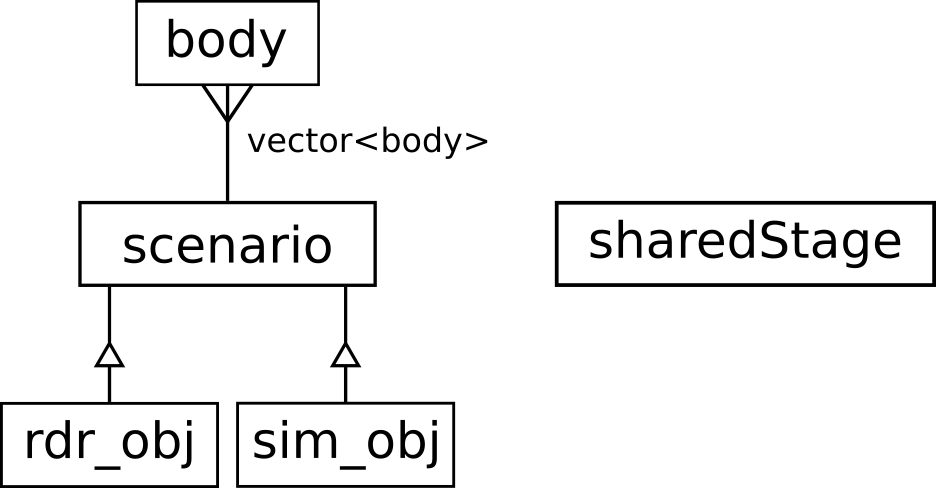
\includegraphics[width=0.8\textwidth]{img/ofd.png}
  \caption{Object Relationship Diagram}
\end{figure}

The object/class structure for this program is extremely basic, and used primarily as the Thread-Local Storage for the separate render and simulation threads. Class Scenario contains a vector consisting of type body, as well as the functions required to manage, return and update the body storage and any other relevant variables, rdrTLC and simTLC (Thread Local Class) will the inherit the scenario class and add on specific functions that pertain to that particular thread.

\paragraph{}
The sharedStage class will contain storage variables similar to the scenario class, however no active management must be carried out in the shared area, which is why it does not inherit the scenario class as it contains functions that allow for the creation or deletion of bodies, scenarios private variables will be 'protected' which allows them to be accessed by the sub-scenario classes that inherit the scenario class.

\subsubsection{body}
\texttt{\lstinputlisting{design/body.hpp}} 

\pagebreak
\subsubsection{scenario}
\texttt{\lstinputlisting{design/scenario.hpp}}
\paragraph{}
The scenario class is designed to be a class template for the Thread-Local Class or Thread-Local Storage for the simulation and rendering threads, the specific classes for which will inherit this class.

\paragraph{}
Other than a body storage vector and the simulation controls, this class also has a status register, this is an 8 bit variable that will be used in a similar fashion to registers in embedded programming, each bit will represent a true / false state and will be used to describe the current state of the executing thread, this is mainly useful for debugging purposes.

\pagebreak
\subsubsection{simTLC}
\texttt{\lstinputlisting{design/simTLC.hpp}}

\subsubsection{rdrTLC}
\texttt{\lstinputlisting{design/rdrTLC.hpp}}

\paragraph{}
Both simTLC and rdrTLC inherit the scenario class, giving them both a body storage vector, simulation control variables and basic public management functions for these variables to keep encapsulation. rdrTLC is very lightweight, including functions that link into the graphics portion, drawBody will draw any particular body given the ID, while draw scene calls drawBody for every body in the store. checkCoord will return the bodyID of a body should one be clicked on.

\paragraph{}
By contrast, simTLC is more complicated, containing functions for dealing with the simulation portion of the program, almost in its entirety. Methods for returning the distance and forces between bodies are the only methods that will return variables, while all other methods make changes to other variables directly. 

\paragraph{}
Forces for every single body relationship for the current iteration will be stored in a single 2D vector matrix, this will be reset and resized at the beginning of every iteration. The forces are stored for both X and Y, split by the diagonal of the same-same relationship. calcForceSum takes all of these relationships and adds them together for each body, putting them into the respective body object in the vector. (scenario) Force calculation is one of the main computational costs in the program.

\paragraph{}
Most actions, such as calculations for velocity, acceleration and position, are all calculated in the body object itself, the functions present in this class are loops to call functions for every body.

\pagebreak
\subsubsection{sharedStage}
\texttt{\lstinputlisting{design/sharedStage.hpp}}

\subsection{Human-Computer Interaction}
\subsubsection{Frame Rate}
\subsubsection{Mock Interface}

\subsection{Testing}
